\documentclass[1p]{elsarticle_modified}
%\bibliographystyle{elsarticle-num}

%\usepackage[colorlinks]{hyperref}
%\usepackage{abbrmath_seonhwa} %\Abb, \Ascr, \Acal ,\Abf, \Afrak
\usepackage{amsfonts}
\usepackage{amssymb}
\usepackage{amsmath}
\usepackage{amsthm}
\usepackage{scalefnt}
\usepackage{amsbsy}
\usepackage{kotex}
\usepackage{caption}
\usepackage{subfig}
\usepackage{color}
\usepackage{graphicx}
\usepackage{xcolor} %% white, black, red, green, blue, cyan, magenta, yellow
\usepackage{float}
\usepackage{setspace}
\usepackage{hyperref}

\usepackage{tikz}
\usetikzlibrary{arrows}

\usepackage{multirow}
\usepackage{array} % fixed length table
\usepackage{hhline}

%%%%%%%%%%%%%%%%%%%%%
\makeatletter
\renewcommand*\env@matrix[1][\arraystretch]{%
	\edef\arraystretch{#1}%
	\hskip -\arraycolsep
	\let\@ifnextchar\new@ifnextchar
	\array{*\c@MaxMatrixCols c}}
\makeatother %https://tex.stackexchange.com/questions/14071/how-can-i-increase-the-line-spacing-in-a-matrix
%%%%%%%%%%%%%%%

\usepackage[normalem]{ulem}

\newcommand{\msout}[1]{\ifmmode\text{\sout{\ensuremath{#1}}}\else\sout{#1}\fi}
%SOURCE: \msout is \stkout macro in https://tex.stackexchange.com/questions/20609/strikeout-in-math-mode

\newcommand{\cancel}[1]{
	\ifmmode
	{\color{red}\msout{#1}}
	\else
	{\color{red}\sout{#1}}
	\fi
}

\newcommand{\add}[1]{
	{\color{blue}\uwave{#1}}
}

\newcommand{\replace}[2]{
	\ifmmode
	{\color{red}\msout{#1}}{\color{blue}\uwave{#2}}
	\else
	{\color{red}\sout{#1}}{\color{blue}\uwave{#2}}
	\fi
}

\newcommand{\Sol}{\mathcal{S}} %segment
\newcommand{\D}{D} %diagram
\newcommand{\A}{\mathcal{A}} %arc


%%%%%%%%%%%%%%%%%%%%%%%%%%%%%5 test

\def\sl{\operatorname{\textup{SL}}(2,\Cbb)}
\def\psl{\operatorname{\textup{PSL}}(2,\Cbb)}
\def\quan{\mkern 1mu \triangleright \mkern 1mu}

\theoremstyle{definition}
\newtheorem{thm}{Theorem}[section]
\newtheorem{prop}[thm]{Proposition}
\newtheorem{lem}[thm]{Lemma}
\newtheorem{ques}[thm]{Question}
\newtheorem{cor}[thm]{Corollary}
\newtheorem{defn}[thm]{Definition}
\newtheorem{exam}[thm]{Example}
\newtheorem{rmk}[thm]{Remark}
\newtheorem{alg}[thm]{Algorithm}

\newcommand{\I}{\sqrt{-1}}
\begin{document}

%\begin{frontmatter}
%
%\title{Boundary parabolic representations of knots up to 8 crossings}
%
%%% Group authors per affiliation:
%\author{Yunhi Cho} 
%\address{Department of Mathematics, University of Seoul, Seoul, Korea}
%\ead{yhcho@uos.ac.kr}
%
%
%\author{Seonhwa Kim} %\fnref{s_kim}}
%\address{Center for Geometry and Physics, Institute for Basic Science, Pohang, 37673, Korea}
%\ead{ryeona17@ibs.re.kr}
%
%\author{Hyuk Kim}
%\address{Department of Mathematical Sciences, Seoul National University, Seoul 08826, Korea}
%\ead{hyukkim@snu.ac.kr}
%
%\author{Seokbeom Yoon}
%\address{Department of Mathematical Sciences, Seoul National University, Seoul, 08826,  Korea}
%\ead{sbyoon15@snu.ac.kr}
%
%\begin{abstract}
%We find all boundary parabolic representation of knots up to 8 crossings.
%
%\end{abstract}
%\begin{keyword}
%    \MSC[2010] 57M25 
%\end{keyword}
%
%\end{frontmatter}

%\linenumbers
%\tableofcontents
%
\newcommand\colored[1]{\textcolor{white}{\rule[-0.35ex]{0.8em}{1.4ex}}\kern-0.8em\color{red} #1}%
%\newcommand\colored[1]{\textcolor{white}{ #1}\kern-2.17ex	\textcolor{white}{ #1}\kern-1.81ex	\textcolor{white}{ #1}\kern-2.15ex\color{red}#1	}

{\Large $\underline{12a_{0446}~(K12a_{0446})}$}

\setlength{\tabcolsep}{10pt}
\renewcommand{\arraystretch}{1.6}
\vspace{1cm}\begin{tabular}{m{100pt}>{\centering\arraybackslash}m{274pt}}
\multirow{5}{120pt}{
	\centering
	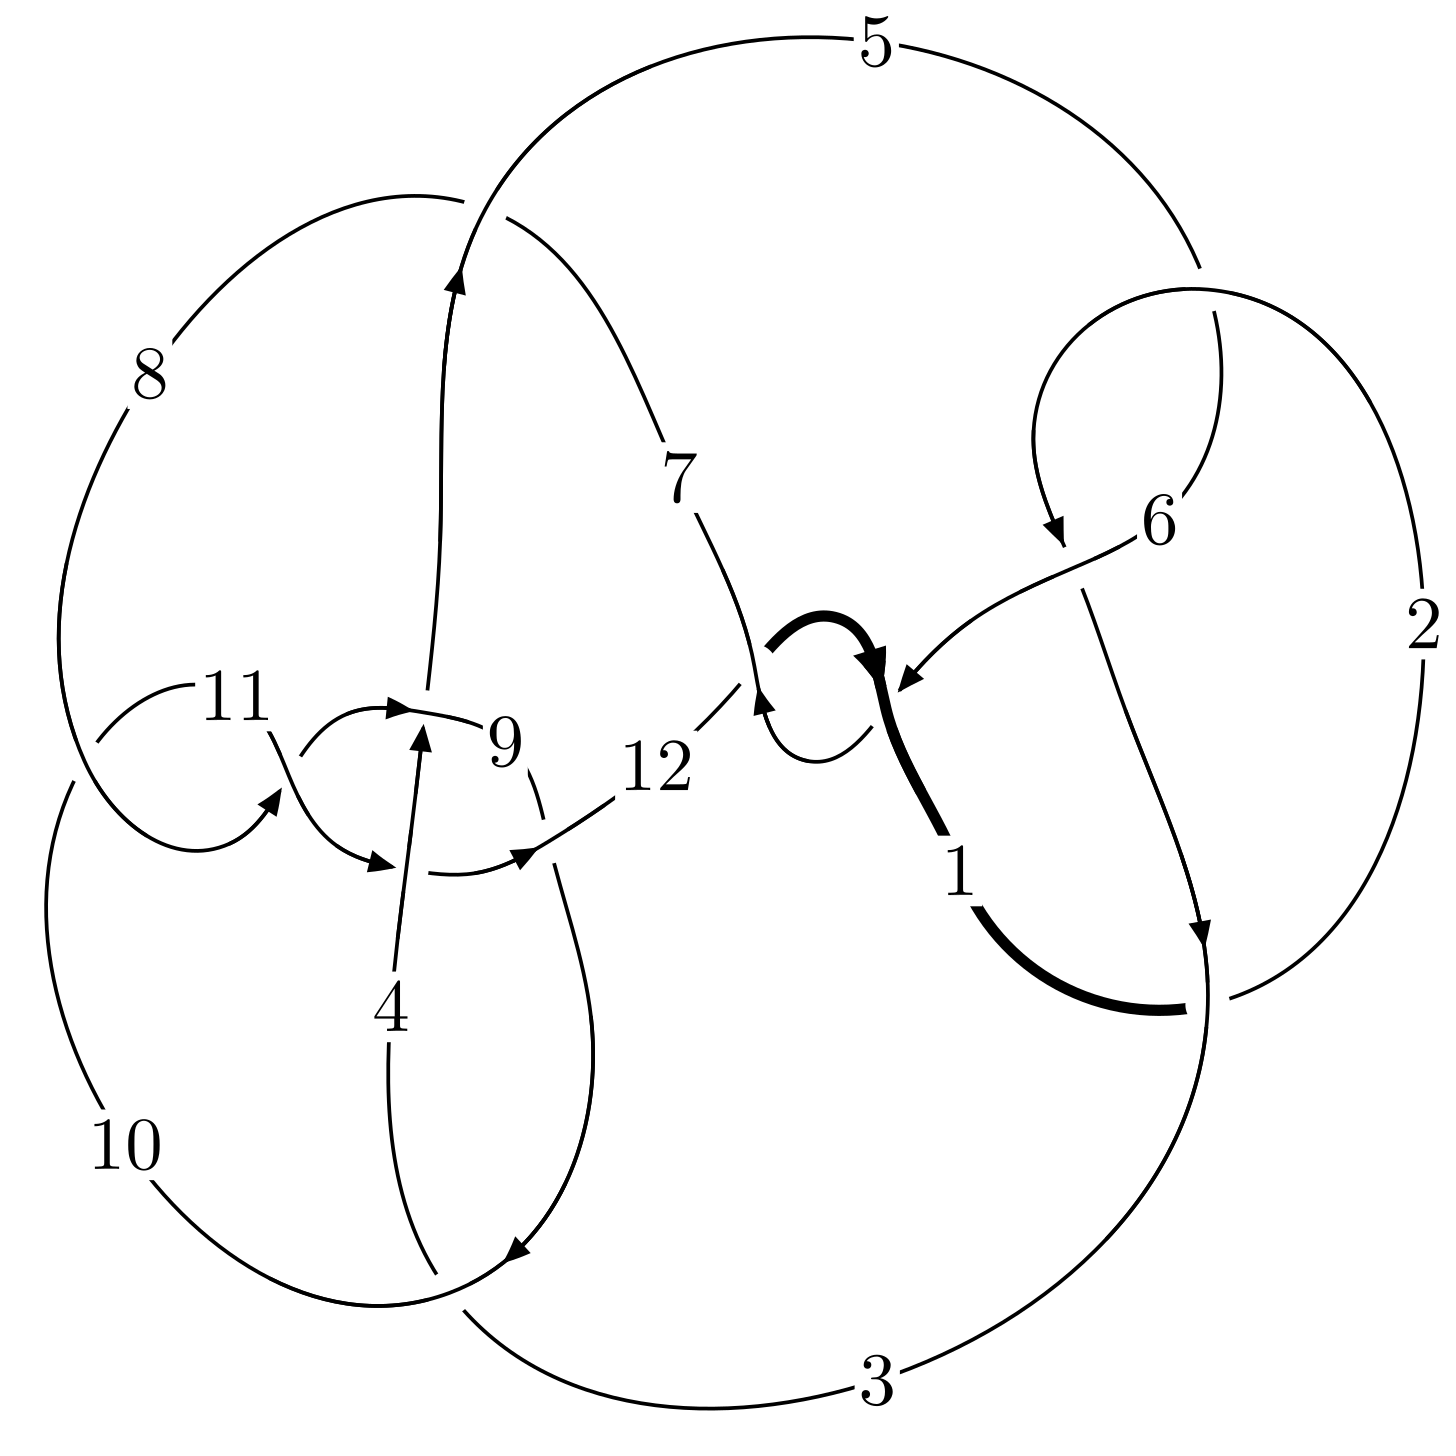
\includegraphics[width=112pt]{../../../GIT/diagram.site/Diagrams/png/1247_12a_0446.png}\\
\ \ \ A knot diagram\footnotemark}&
\allowdisplaybreaks
\textbf{Linearized knot diagam} \\
\cline{2-2}
 &
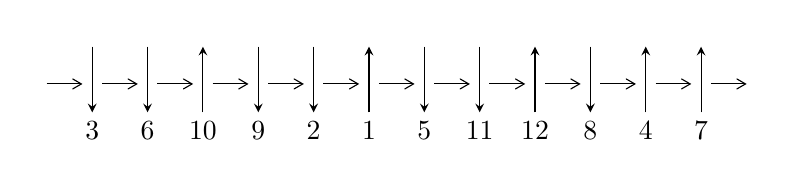
\begin{tikzpicture}[x=20pt, y=17pt]
	% nodes
	\node (C0) at (0, 0) {};
	\node (C1) at (1, 0) {};
	\node (C1U) at (1, +1) {};
	\node (C1D) at (1, -1) {3};

	\node (C2) at (2, 0) {};
	\node (C2U) at (2, +1) {};
	\node (C2D) at (2, -1) {6};

	\node (C3) at (3, 0) {};
	\node (C3U) at (3, +1) {};
	\node (C3D) at (3, -1) {10};

	\node (C4) at (4, 0) {};
	\node (C4U) at (4, +1) {};
	\node (C4D) at (4, -1) {9};

	\node (C5) at (5, 0) {};
	\node (C5U) at (5, +1) {};
	\node (C5D) at (5, -1) {2};

	\node (C6) at (6, 0) {};
	\node (C6U) at (6, +1) {};
	\node (C6D) at (6, -1) {1};

	\node (C7) at (7, 0) {};
	\node (C7U) at (7, +1) {};
	\node (C7D) at (7, -1) {5};

	\node (C8) at (8, 0) {};
	\node (C8U) at (8, +1) {};
	\node (C8D) at (8, -1) {11};

	\node (C9) at (9, 0) {};
	\node (C9U) at (9, +1) {};
	\node (C9D) at (9, -1) {12};

	\node (C10) at (10, 0) {};
	\node (C10U) at (10, +1) {};
	\node (C10D) at (10, -1) {8};

	\node (C11) at (11, 0) {};
	\node (C11U) at (11, +1) {};
	\node (C11D) at (11, -1) {4};

	\node (C12) at (12, 0) {};
	\node (C12U) at (12, +1) {};
	\node (C12D) at (12, -1) {7};
	\node (C13) at (13, 0) {};

	% arrows
	\draw[->,>={angle 60}]
	(C0) edge (C1) (C1) edge (C2) (C2) edge (C3) (C3) edge (C4) (C4) edge (C5) (C5) edge (C6) (C6) edge (C7) (C7) edge (C8) (C8) edge (C9) (C9) edge (C10) (C10) edge (C11) (C11) edge (C12) (C12) edge (C13) ;	\draw[->,>=stealth]
	(C1U) edge (C1D) (C2U) edge (C2D) (C3D) edge (C3U) (C4U) edge (C4D) (C5U) edge (C5D) (C6D) edge (C6U) (C7U) edge (C7D) (C8U) edge (C8D) (C9D) edge (C9U) (C10U) edge (C10D) (C11D) edge (C11U) (C12D) edge (C12U) ;
	\end{tikzpicture} \\
\hhline{~~} \\& 
\textbf{Solving Sequence} \\ \cline{2-2} 
 &
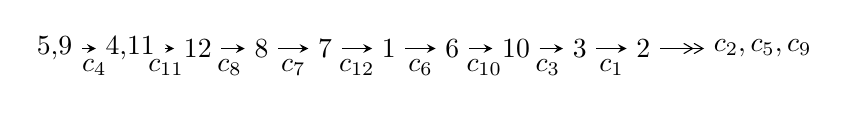
\begin{tikzpicture}[x=23pt, y=7pt]
	% node
	\node (A0) at (-1/8, 0) {5,9};
	\node (A1) at (17/16, 0) {4,11};
	\node (A2) at (17/8, 0) {12};
	\node (A3) at (25/8, 0) {8};
	\node (A4) at (33/8, 0) {7};
	\node (A5) at (41/8, 0) {1};
	\node (A6) at (49/8, 0) {6};
	\node (A7) at (57/8, 0) {10};
	\node (A8) at (65/8, 0) {3};
	\node (A9) at (73/8, 0) {2};
	\node (C1) at (1/2, -1) {$c_{4}$};
	\node (C2) at (13/8, -1) {$c_{11}$};
	\node (C3) at (21/8, -1) {$c_{8}$};
	\node (C4) at (29/8, -1) {$c_{7}$};
	\node (C5) at (37/8, -1) {$c_{12}$};
	\node (C6) at (45/8, -1) {$c_{6}$};
	\node (C7) at (53/8, -1) {$c_{10}$};
	\node (C8) at (61/8, -1) {$c_{3}$};
	\node (C9) at (69/8, -1) {$c_{1}$};
	\node (A10) at (11, 0) {$c_{2},c_{5},c_{9}$};

	% edge
	\draw[->,>=stealth]	
	(A0) edge (A1) (A1) edge (A2) (A2) edge (A3) (A3) edge (A4) (A4) edge (A5) (A5) edge (A6) (A6) edge (A7) (A7) edge (A8) (A8) edge (A9) ;
	\draw[->>,>={angle 60}]	
	(A9) edge (A10);
\end{tikzpicture} \\ 

\end{tabular} \\

\footnotetext{
The image of knot diagram is generated by the software ``\textbf{Draw programme}" developed by Andrew Bartholomew(\url{http://www.layer8.co.uk/maths/draw/index.htm\#Running-draw}), where we modified some parts for our purpose(\url{https://github.com/CATsTAILs/LinksPainter}).
}\phantom \\ \newline 
\centering \textbf{Ideals for irreducible components\footnotemark of $X_{\text{par}}$} 
 
\begin{align*}
I^u_{1}&=\langle 
9.81367\times10^{890} u^{115}-1.43266\times10^{891} u^{114}+\cdots+4.70124\times10^{891} b-1.58539\times10^{893},\\
\phantom{I^u_{1}}&\phantom{= \langle  }1.01422\times10^{893} u^{115}-1.53993\times10^{893} u^{114}+\cdots+3.71398\times10^{893} a-1.36518\times10^{895},\\
\phantom{I^u_{1}}&\phantom{= \langle  }u^{116}-2 u^{115}+\cdots+115 u+79\rangle \\
I^u_{2}&=\langle 
b+2,\;a-1,\;u+1\rangle \\
\\
\end{align*}
\raggedright * 2 irreducible components of $\dim_{\mathbb{C}}=0$, with total 117 representations.\\
\footnotetext{All coefficients of polynomials are rational numbers. But the coefficients are sometimes approximated in decimal forms when there is not enough margin.}
\newpage
\renewcommand{\arraystretch}{1}
\centering \section*{I. $I^u_{1}= \langle 9.81\times10^{890} u^{115}-1.43\times10^{891} u^{114}+\cdots+4.70\times10^{891} b-1.59\times10^{893},\;1.01\times10^{893} u^{115}-1.54\times10^{893} u^{114}+\cdots+3.71\times10^{893} a-1.37\times10^{895},\;u^{116}-2 u^{115}+\cdots+115 u+79 \rangle$}
\flushleft \textbf{(i) Arc colorings}\\
\begin{tabular}{m{7pt} m{180pt} m{7pt} m{180pt} }
\flushright $a_{5}=$&$\begin{pmatrix}1\\0\end{pmatrix}$ \\
\flushright $a_{9}=$&$\begin{pmatrix}0\\u\end{pmatrix}$ \\
\flushright $a_{4}=$&$\begin{pmatrix}1\\- u^2\end{pmatrix}$ \\
\flushright $a_{11}=$&$\begin{pmatrix}-0.273081 u^{115}+0.414631 u^{114}+\cdots+122.190 u+36.7579\\-0.208746 u^{115}+0.304741 u^{114}+\cdots+103.296 u+33.7227\end{pmatrix}$ \\
\flushright $a_{12}=$&$\begin{pmatrix}-0.552619 u^{115}+0.826356 u^{114}+\cdots+262.185 u+80.8716\\-0.135003 u^{115}+0.194749 u^{114}+\cdots+64.2667 u+22.0820\end{pmatrix}$ \\
\flushright $a_{8}=$&$\begin{pmatrix}0.813970 u^{115}-1.20617 u^{114}+\cdots-380.866 u-124.597\\0.218953 u^{115}-0.325444 u^{114}+\cdots-108.758 u-30.6043\end{pmatrix}$ \\
\flushright $a_{7}=$&$\begin{pmatrix}1.03292 u^{115}-1.53161 u^{114}+\cdots-489.624 u-155.202\\0.218953 u^{115}-0.325444 u^{114}+\cdots-108.758 u-30.6043\end{pmatrix}$ \\
\flushright $a_{1}=$&$\begin{pmatrix}0.629874 u^{115}-0.885124 u^{114}+\cdots-213.206 u-79.4249\\-0.745206 u^{115}+1.10942 u^{114}+\cdots+382.947 u+115.904\end{pmatrix}$ \\
\flushright $a_{6}=$&$\begin{pmatrix}-2.77476 u^{115}+4.16315 u^{114}+\cdots+1499.26 u+434.932\\0.559144 u^{115}-0.858928 u^{114}+\cdots-344.823 u-93.2392\end{pmatrix}$ \\
\flushright $a_{10}=$&$\begin{pmatrix}1.64280 u^{115}-2.44093 u^{114}+\cdots-803.107 u-247.103\\-0.0368661 u^{115}+0.0591602 u^{114}+\cdots+28.2441 u+8.14818\end{pmatrix}$ \\
\flushright $a_{3}=$&$\begin{pmatrix}0.686595 u^{115}-0.996166 u^{114}+\cdots-302.971 u-97.1620\\-0.447903 u^{115}+0.662858 u^{114}+\cdots+223.489 u+67.8492\end{pmatrix}$ \\
\flushright $a_{2}=$&$\begin{pmatrix}2.40163 u^{115}-3.68546 u^{114}+\cdots-1480.26 u-410.550\\-0.0391826 u^{115}+0.0512360 u^{114}+\cdots+4.80775 u+4.71164\end{pmatrix}$\\&\end{tabular}
\flushleft \textbf{(ii) Obstruction class $= -1$}\\~\\
\flushleft \textbf{(iii) Cusp Shapes $= 1.88684 u^{115}-2.93040 u^{114}+\cdots-1183.32 u-304.174$}\\~\\
\newpage\renewcommand{\arraystretch}{1}
\flushleft \textbf{(iv) u-Polynomials at the component}\newline \\
\begin{tabular}{m{50pt}|m{274pt}}
Crossings & \hspace{64pt}u-Polynomials at each crossing \\
\hline $$\begin{aligned}c_{1}\end{aligned}$$&$\begin{aligned}
&u^{116}+62 u^{115}+\cdots- u+1
\end{aligned}$\\
\hline $$\begin{aligned}c_{2},c_{5}\end{aligned}$$&$\begin{aligned}
&u^{116}+2 u^{115}+\cdots+5 u+1
\end{aligned}$\\
\hline $$\begin{aligned}c_{3}\end{aligned}$$&$\begin{aligned}
&u^{116}-51 u^{114}+\cdots-208 u-56
\end{aligned}$\\
\hline $$\begin{aligned}c_{4}\end{aligned}$$&$\begin{aligned}
&u^{116}+2 u^{115}+\cdots-115 u+79
\end{aligned}$\\
\hline $$\begin{aligned}c_{6},c_{12}\end{aligned}$$&$\begin{aligned}
&u^{116}+3 u^{115}+\cdots+565 u^2-32
\end{aligned}$\\
\hline $$\begin{aligned}c_{7}\end{aligned}$$&$\begin{aligned}
&u^{116}-12 u^{115}+\cdots-1181 u+29
\end{aligned}$\\
\hline $$\begin{aligned}c_{8},c_{10}\end{aligned}$$&$\begin{aligned}
&u^{116}-2 u^{115}+\cdots- u-1
\end{aligned}$\\
\hline $$\begin{aligned}c_{9}\end{aligned}$$&$\begin{aligned}
&u^{116}+19 u^{115}+\cdots-2 u+2
\end{aligned}$\\
\hline $$\begin{aligned}c_{11}\end{aligned}$$&$\begin{aligned}
&u^{116}-2 u^{115}+\cdots+u-1
\end{aligned}$\\
\hline
\end{tabular}\\~\\
\newpage\renewcommand{\arraystretch}{1}
\flushleft \textbf{(v) Riley Polynomials at the component}\newline \\
\begin{tabular}{m{50pt}|m{274pt}}
Crossings & \hspace{64pt}Riley Polynomials at each crossing \\
\hline $$\begin{aligned}c_{1}\end{aligned}$$&$\begin{aligned}
&y^{116}-14 y^{115}+\cdots+69 y+1
\end{aligned}$\\
\hline $$\begin{aligned}c_{2},c_{5}\end{aligned}$$&$\begin{aligned}
&y^{116}-62 y^{115}+\cdots+y+1
\end{aligned}$\\
\hline $$\begin{aligned}c_{3}\end{aligned}$$&$\begin{aligned}
&y^{116}-102 y^{115}+\cdots+113760 y+3136
\end{aligned}$\\
\hline $$\begin{aligned}c_{4}\end{aligned}$$&$\begin{aligned}
&y^{116}-122 y^{115}+\cdots-263971 y+6241
\end{aligned}$\\
\hline $$\begin{aligned}c_{6},c_{12}\end{aligned}$$&$\begin{aligned}
&y^{116}+87 y^{115}+\cdots-36160 y+1024
\end{aligned}$\\
\hline $$\begin{aligned}c_{7}\end{aligned}$$&$\begin{aligned}
&y^{116}+22 y^{115}+\cdots+2701257 y+841
\end{aligned}$\\
\hline $$\begin{aligned}c_{8},c_{10}\end{aligned}$$&$\begin{aligned}
&y^{116}-74 y^{115}+\cdots-107 y+1
\end{aligned}$\\
\hline $$\begin{aligned}c_{9}\end{aligned}$$&$\begin{aligned}
&y^{116}-9 y^{115}+\cdots-88 y+4
\end{aligned}$\\
\hline $$\begin{aligned}c_{11}\end{aligned}$$&$\begin{aligned}
&y^{116}+18 y^{115}+\cdots+y+1
\end{aligned}$\\
\hline
\end{tabular}\\~\\
\newpage\flushleft \textbf{(vi) Complex Volumes and Cusp Shapes}
$$\begin{array}{c|c|c}  
\text{Solutions to }I^u_{1}& \I (\text{vol} + \sqrt{-1}CS) & \text{Cusp shape}\\
 \hline 
\begin{aligned}
u &= \phantom{-}0.951325 + 0.313588 I \\
a &= -1.225350 - 0.298169 I \\
b &= \phantom{-}1.137870 + 0.252464 I\end{aligned}
 & -1.01973 - 1.06715 I & \phantom{-0.000000 } 0 \\ \hline\begin{aligned}
u &= \phantom{-}0.951325 - 0.313588 I \\
a &= -1.225350 + 0.298169 I \\
b &= \phantom{-}1.137870 - 0.252464 I\end{aligned}
 & -1.01973 + 1.06715 I & \phantom{-0.000000 } 0 \\ \hline\begin{aligned}
u &= -0.596448 + 0.824284 I \\
a &= \phantom{-}0.743724 - 0.759157 I \\
b &= \phantom{-}0.218175 - 0.249595 I\end{aligned}
 & \phantom{-}3.93410 + 2.59183 I & \phantom{-0.000000 } 0 \\ \hline\begin{aligned}
u &= -0.596448 - 0.824284 I \\
a &= \phantom{-}0.743724 + 0.759157 I \\
b &= \phantom{-}0.218175 + 0.249595 I\end{aligned}
 & \phantom{-}3.93410 - 2.59183 I & \phantom{-0.000000 } 0 \\ \hline\begin{aligned}
u &= -0.952880 + 0.239211 I \\
a &= \phantom{-}1.349090 - 0.420028 I \\
b &= -1.265490 + 0.213892 I\end{aligned}
 & -1.45435 + 5.15444 I & \phantom{-0.000000 } 0 \\ \hline\begin{aligned}
u &= -0.952880 - 0.239211 I \\
a &= \phantom{-}1.349090 + 0.420028 I \\
b &= -1.265490 - 0.213892 I\end{aligned}
 & -1.45435 - 5.15444 I & \phantom{-0.000000 } 0 \\ \hline\begin{aligned}
u &= \phantom{-}0.084892 + 1.020460 I \\
a &= \phantom{-}0.219707 - 0.594375 I \\
b &= -0.130857 + 0.587100 I\end{aligned}
 & \phantom{-}2.67777 - 2.30723 I & \phantom{-0.000000 } 0 \\ \hline\begin{aligned}
u &= \phantom{-}0.084892 - 1.020460 I \\
a &= \phantom{-}0.219707 + 0.594375 I \\
b &= -0.130857 - 0.587100 I\end{aligned}
 & \phantom{-}2.67777 + 2.30723 I & \phantom{-0.000000 } 0 \\ \hline\begin{aligned}
u &= \phantom{-}0.957748 + 0.114531 I \\
a &= -1.48224 - 0.63128 I \\
b &= \phantom{-}1.48514 + 0.08966 I\end{aligned}
 & -7.51968 - 10.06630 I & \phantom{-0.000000 } 0 \\ \hline\begin{aligned}
u &= \phantom{-}0.957748 - 0.114531 I \\
a &= -1.48224 + 0.63128 I \\
b &= \phantom{-}1.48514 - 0.08966 I\end{aligned}
 & -7.51968 + 10.06630 I & \phantom{-0.000000 } 0\\
 \hline 
 \end{array}$$\newpage$$\begin{array}{c|c|c}  
\text{Solutions to }I^u_{1}& \I (\text{vol} + \sqrt{-1}CS) & \text{Cusp shape}\\
 \hline 
\begin{aligned}
u &= \phantom{-}0.380130 + 0.969615 I \\
a &= \phantom{-}0.570001 - 0.668737 I \\
b &= -0.642625 + 0.438196 I\end{aligned}
 & \phantom{-}0.56321 - 3.80754 I & \phantom{-0.000000 } 0 \\ \hline\begin{aligned}
u &= \phantom{-}0.380130 - 0.969615 I \\
a &= \phantom{-}0.570001 + 0.668737 I \\
b &= -0.642625 - 0.438196 I\end{aligned}
 & \phantom{-}0.56321 + 3.80754 I & \phantom{-0.000000 } 0 \\ \hline\begin{aligned}
u &= \phantom{-}0.064129 + 1.043420 I \\
a &= -0.150013 - 0.358017 I \\
b &= -0.005139 + 0.568167 I\end{aligned}
 & \phantom{-}2.59093 - 2.28064 I & \phantom{-0.000000 } 0 \\ \hline\begin{aligned}
u &= \phantom{-}0.064129 - 1.043420 I \\
a &= -0.150013 + 0.358017 I \\
b &= -0.005139 - 0.568167 I\end{aligned}
 & \phantom{-}2.59093 + 2.28064 I & \phantom{-0.000000 } 0 \\ \hline\begin{aligned}
u &= \phantom{-}0.881712 + 0.572493 I \\
a &= -0.979523 + 0.283828 I \\
b &= \phantom{-}0.978600 + 0.277804 I\end{aligned}
 & -1.90994 - 0.93281 I & \phantom{-0.000000 } 0 \\ \hline\begin{aligned}
u &= \phantom{-}0.881712 - 0.572493 I \\
a &= -0.979523 - 0.283828 I \\
b &= \phantom{-}0.978600 - 0.277804 I\end{aligned}
 & -1.90994 + 0.93281 I & \phantom{-0.000000 } 0 \\ \hline\begin{aligned}
u &= \phantom{-}0.711364 + 0.627206 I \\
a &= -0.672678 - 0.684854 I \\
b &= \phantom{-}0.152953 + 0.002754 I\end{aligned}
 & -1.06556 - 3.75617 I & \phantom{-0.000000 } 0 \\ \hline\begin{aligned}
u &= \phantom{-}0.711364 - 0.627206 I \\
a &= -0.672678 + 0.684854 I \\
b &= \phantom{-}0.152953 - 0.002754 I\end{aligned}
 & -1.06556 + 3.75617 I & \phantom{-0.000000 } 0 \\ \hline\begin{aligned}
u &= -0.936756 + 0.131580 I \\
a &= \phantom{-}1.50411 - 0.58305 I \\
b &= -1.42992 + 0.07583 I\end{aligned}
 & -4.43225 + 5.33303 I & \phantom{-0.000000 } 0 \\ \hline\begin{aligned}
u &= -0.936756 - 0.131580 I \\
a &= \phantom{-}1.50411 + 0.58305 I \\
b &= -1.42992 - 0.07583 I\end{aligned}
 & -4.43225 - 5.33303 I & \phantom{-0.000000 } 0\\
 \hline 
 \end{array}$$\newpage$$\begin{array}{c|c|c}  
\text{Solutions to }I^u_{1}& \I (\text{vol} + \sqrt{-1}CS) & \text{Cusp shape}\\
 \hline 
\begin{aligned}
u &= \phantom{-}0.964220 + 0.438444 I \\
a &= -0.793334 - 0.454170 I \\
b &= \phantom{-}0.701814 + 0.332184 I\end{aligned}
 & -2.45699 - 1.34404 I & \phantom{-0.000000 } 0 \\ \hline\begin{aligned}
u &= \phantom{-}0.964220 - 0.438444 I \\
a &= -0.793334 + 0.454170 I \\
b &= \phantom{-}0.701814 - 0.332184 I\end{aligned}
 & -2.45699 + 1.34404 I & \phantom{-0.000000 } 0 \\ \hline\begin{aligned}
u &= \phantom{-}0.646590 + 0.851847 I \\
a &= -0.752328 - 0.742271 I \\
b &= -0.294950 - 0.151308 I\end{aligned}
 & \phantom{-}3.53389 - 7.04008 I & \phantom{-0.000000 } 0 \\ \hline\begin{aligned}
u &= \phantom{-}0.646590 - 0.851847 I \\
a &= -0.752328 + 0.742271 I \\
b &= -0.294950 + 0.151308 I\end{aligned}
 & \phantom{-}3.53389 + 7.04008 I & \phantom{-0.000000 } 0 \\ \hline\begin{aligned}
u &= \phantom{-}0.909971 + 0.102992 I \\
a &= -1.57919 - 0.61335 I \\
b &= \phantom{-}1.44161 - 0.00386 I\end{aligned}
 & -8.34099 - 1.39112 I & \phantom{-0.000000 } 0 \\ \hline\begin{aligned}
u &= \phantom{-}0.909971 - 0.102992 I \\
a &= -1.57919 + 0.61335 I \\
b &= \phantom{-}1.44161 + 0.00386 I\end{aligned}
 & -8.34099 + 1.39112 I & \phantom{-0.000000 } 0 \\ \hline\begin{aligned}
u &= -0.969402 + 0.494770 I \\
a &= \phantom{-}0.794653 - 0.526373 I \\
b &= -0.578732 + 0.423782 I\end{aligned}
 & -5.94980 + 5.43731 I & \phantom{-0.000000 } 0 \\ \hline\begin{aligned}
u &= -0.969402 - 0.494770 I \\
a &= \phantom{-}0.794653 + 0.526373 I \\
b &= -0.578732 - 0.423782 I\end{aligned}
 & -5.94980 - 5.43731 I & \phantom{-0.000000 } 0 \\ \hline\begin{aligned}
u &= -0.468281 + 0.990716 I \\
a &= \phantom{-}0.232120 - 0.155624 I \\
b &= -0.044643 + 0.762341 I\end{aligned}
 & -4.00401 - 0.60060 I & \phantom{-0.000000 } 0 \\ \hline\begin{aligned}
u &= -0.468281 - 0.990716 I \\
a &= \phantom{-}0.232120 + 0.155624 I \\
b &= -0.044643 - 0.762341 I\end{aligned}
 & -4.00401 + 0.60060 I & \phantom{-0.000000 } 0\\
 \hline 
 \end{array}$$\newpage$$\begin{array}{c|c|c}  
\text{Solutions to }I^u_{1}& \I (\text{vol} + \sqrt{-1}CS) & \text{Cusp shape}\\
 \hline 
\begin{aligned}
u &= -1.010200 + 0.443183 I \\
a &= \phantom{-}0.862881 - 0.480901 I \\
b &= -0.762564 + 0.458627 I\end{aligned}
 & -5.62707 - 3.04654 I & \phantom{-0.000000 } 0 \\ \hline\begin{aligned}
u &= -1.010200 - 0.443183 I \\
a &= \phantom{-}0.862881 + 0.480901 I \\
b &= -0.762564 - 0.458627 I\end{aligned}
 & -5.62707 + 3.04654 I & \phantom{-0.000000 } 0 \\ \hline\begin{aligned}
u &= \phantom{-}0.346639 + 1.056800 I \\
a &= -0.227147 - 0.202967 I \\
b &= -0.027442 + 0.697767 I\end{aligned}
 & -0.06123 - 3.10256 I & \phantom{-0.000000 } 0 \\ \hline\begin{aligned}
u &= \phantom{-}0.346639 - 1.056800 I \\
a &= -0.227147 + 0.202967 I \\
b &= -0.027442 - 0.697767 I\end{aligned}
 & -0.06123 + 3.10256 I & \phantom{-0.000000 } 0 \\ \hline\begin{aligned}
u &= -0.495663 + 0.730134 I \\
a &= \phantom{-}0.708823 - 0.811665 I \\
b &= -0.008967 - 0.405619 I\end{aligned}
 & \phantom{-}2.39643 + 1.55166 I & \phantom{-0.000000 } 0 \\ \hline\begin{aligned}
u &= -0.495663 - 0.730134 I \\
a &= \phantom{-}0.708823 + 0.811665 I \\
b &= -0.008967 + 0.405619 I\end{aligned}
 & \phantom{-}2.39643 - 1.55166 I & \phantom{-0.000000 } 0 \\ \hline\begin{aligned}
u &= \phantom{-}0.739644 + 0.865988 I \\
a &= -0.760142 - 0.718167 I \\
b &= -0.349873 + 0.057411 I\end{aligned}
 & \phantom{-}0.44560 - 7.70285 I & \phantom{-0.000000 } 0 \\ \hline\begin{aligned}
u &= \phantom{-}0.739644 - 0.865988 I \\
a &= -0.760142 + 0.718167 I \\
b &= -0.349873 - 0.057411 I\end{aligned}
 & \phantom{-}0.44560 + 7.70285 I & \phantom{-0.000000 } 0 \\ \hline\begin{aligned}
u &= -0.768688 + 0.842410 I \\
a &= \phantom{-}0.757586 - 0.709448 I \\
b &= \phantom{-}0.298085 + 0.128897 I\end{aligned}
 & -3.60377 + 3.86288 I & \phantom{-0.000000 } 0 \\ \hline\begin{aligned}
u &= -0.768688 - 0.842410 I \\
a &= \phantom{-}0.757586 + 0.709448 I \\
b &= \phantom{-}0.298085 - 0.128897 I\end{aligned}
 & -3.60377 - 3.86288 I & \phantom{-0.000000 } 0\\
 \hline 
 \end{array}$$\newpage$$\begin{array}{c|c|c}  
\text{Solutions to }I^u_{1}& \I (\text{vol} + \sqrt{-1}CS) & \text{Cusp shape}\\
 \hline 
\begin{aligned}
u &= \phantom{-}0.408925 + 0.752776 I \\
a &= -0.739911 - 0.853696 I \\
b &= \phantom{-}0.019426 - 0.574858 I\end{aligned}
 & -0.14534 + 2.85221 I & \phantom{-0.000000 } 0 \\ \hline\begin{aligned}
u &= \phantom{-}0.408925 - 0.752776 I \\
a &= -0.739911 + 0.853696 I \\
b &= \phantom{-}0.019426 + 0.574858 I\end{aligned}
 & -0.14534 - 2.85221 I & \phantom{-0.000000 } 0 \\ \hline\begin{aligned}
u &= -0.481940 + 1.043550 I \\
a &= -0.626250 - 0.573662 I \\
b &= \phantom{-}0.720874 + 0.197474 I\end{aligned}
 & -1.90960 + 8.56015 I & \phantom{-0.000000 } 0 \\ \hline\begin{aligned}
u &= -0.481940 - 1.043550 I \\
a &= -0.626250 + 0.573662 I \\
b &= \phantom{-}0.720874 - 0.197474 I\end{aligned}
 & -1.90960 - 8.56015 I & \phantom{-0.000000 } 0 \\ \hline\begin{aligned}
u &= -0.752662 + 0.886476 I \\
a &= \phantom{-}0.765501 - 0.716826 I \\
b &= \phantom{-}0.400952 + 0.084836 I\end{aligned}
 & -2.56650 + 12.52600 I & \phantom{-0.000000 } 0 \\ \hline\begin{aligned}
u &= -0.752662 - 0.886476 I \\
a &= \phantom{-}0.765501 + 0.716826 I \\
b &= \phantom{-}0.400952 - 0.084836 I\end{aligned}
 & -2.56650 - 12.52600 I & \phantom{-0.000000 } 0 \\ \hline\begin{aligned}
u &= -0.409179 + 0.700700 I \\
a &= -0.795198 - 0.929070 I \\
b &= \phantom{-}1.029620 + 0.902177 I\end{aligned}
 & -3.81251 + 0.96684 I & \phantom{-0.000000 } 0 \\ \hline\begin{aligned}
u &= -0.409179 - 0.700700 I \\
a &= -0.795198 + 0.929070 I \\
b &= \phantom{-}1.029620 - 0.902177 I\end{aligned}
 & -3.81251 - 0.96684 I & \phantom{-0.000000 } 0 \\ \hline\begin{aligned}
u &= \phantom{-}1.026410 + 0.602938 I \\
a &= \phantom{-}1.054580 - 0.358615 I \\
b &= -2.22047 + 0.23273 I\end{aligned}
 & -11.34380 - 0.03428 I & \phantom{-0.000000 } 0 \\ \hline\begin{aligned}
u &= \phantom{-}1.026410 - 0.602938 I \\
a &= \phantom{-}1.054580 + 0.358615 I \\
b &= -2.22047 - 0.23273 I\end{aligned}
 & -11.34380 + 0.03428 I & \phantom{-0.000000 } 0\\
 \hline 
 \end{array}$$\newpage$$\begin{array}{c|c|c}  
\text{Solutions to }I^u_{1}& \I (\text{vol} + \sqrt{-1}CS) & \text{Cusp shape}\\
 \hline 
\begin{aligned}
u &= -0.385613 + 1.128150 I \\
a &= \phantom{-}0.256170 - 0.201485 I \\
b &= \phantom{-}0.072518 + 0.735096 I\end{aligned}
 & -2.98922 + 7.86043 I & \phantom{-0.000000 } 0 \\ \hline\begin{aligned}
u &= -0.385613 - 1.128150 I \\
a &= \phantom{-}0.256170 + 0.201485 I \\
b &= \phantom{-}0.072518 - 0.735096 I\end{aligned}
 & -2.98922 - 7.86043 I & \phantom{-0.000000 } 0 \\ \hline\begin{aligned}
u &= -1.032620 + 0.660866 I \\
a &= -1.018910 - 0.361684 I \\
b &= \phantom{-}2.16318 + 0.12160 I\end{aligned}
 & -7.73953 + 4.64372 I & \phantom{-0.000000 } 0 \\ \hline\begin{aligned}
u &= -1.032620 - 0.660866 I \\
a &= -1.018910 + 0.361684 I \\
b &= \phantom{-}2.16318 - 0.12160 I\end{aligned}
 & -7.73953 - 4.64372 I & \phantom{-0.000000 } 0 \\ \hline\begin{aligned}
u &= -0.710479 + 0.194269 I \\
a &= \phantom{-}1.94994 - 0.14929 I \\
b &= -1.075650 - 0.138829 I\end{aligned}
 & -4.93169 + 1.71660 I & \phantom{-0.000000 } 0 \\ \hline\begin{aligned}
u &= -0.710479 - 0.194269 I \\
a &= \phantom{-}1.94994 + 0.14929 I \\
b &= -1.075650 + 0.138829 I\end{aligned}
 & -4.93169 - 1.71660 I & \phantom{-0.000000 } 0 \\ \hline\begin{aligned}
u &= \phantom{-}1.089870 + 0.664564 I \\
a &= \phantom{-}1.011240 - 0.329764 I \\
b &= -2.26352 + 0.04611 I\end{aligned}
 & -11.4429 - 9.1627 I & \phantom{-0.000000 } 0 \\ \hline\begin{aligned}
u &= \phantom{-}1.089870 - 0.664564 I \\
a &= \phantom{-}1.011240 + 0.329764 I \\
b &= -2.26352 - 0.04611 I\end{aligned}
 & -11.4429 + 9.1627 I & \phantom{-0.000000 } 0 \\ \hline\begin{aligned}
u &= \phantom{-}0.631956 + 0.275564 I \\
a &= -0.182383 + 0.087700 I \\
b &= \phantom{-}0.495068 + 0.435356 I\end{aligned}
 & -1.47021 - 0.27681 I & \phantom{-0.000000 } 0 \\ \hline\begin{aligned}
u &= \phantom{-}0.631956 - 0.275564 I \\
a &= -0.182383 - 0.087700 I \\
b &= \phantom{-}0.495068 - 0.435356 I\end{aligned}
 & -1.47021 + 0.27681 I & \phantom{-0.000000 } 0\\
 \hline 
 \end{array}$$\newpage$$\begin{array}{c|c|c}  
\text{Solutions to }I^u_{1}& \I (\text{vol} + \sqrt{-1}CS) & \text{Cusp shape}\\
 \hline 
\begin{aligned}
u &= \phantom{-}0.268648 + 0.573440 I \\
a &= -0.680616 - 1.049200 I \\
b &= \phantom{-}0.412706 - 0.654226 I\end{aligned}
 & -0.57611 - 4.58827 I & \phantom{-0.000000 -}0. + 4.86927 I \\ \hline\begin{aligned}
u &= \phantom{-}0.268648 - 0.573440 I \\
a &= -0.680616 + 1.049200 I \\
b &= \phantom{-}0.412706 + 0.654226 I\end{aligned}
 & -0.57611 + 4.58827 I & \phantom{-0.000000 } 0. - 4.86927 I \\ \hline\begin{aligned}
u &= -0.96196 + 1.05654 I \\
a &= -0.812469 - 0.370562 I \\
b &= \phantom{-}1.49889 - 0.49595 I\end{aligned}
 & -2.79197 + 2.22125 I & \phantom{-0.000000 } 0 \\ \hline\begin{aligned}
u &= -0.96196 - 1.05654 I \\
a &= -0.812469 + 0.370562 I \\
b &= \phantom{-}1.49889 + 0.49595 I\end{aligned}
 & -2.79197 - 2.22125 I & \phantom{-0.000000 } 0 \\ \hline\begin{aligned}
u &= \phantom{-}0.492095 + 0.287973 I \\
a &= \phantom{-}1.89019 - 0.51259 I \\
b &= -1.86100 - 1.33877 I\end{aligned}
 & -5.51335 - 10.68540 I & -6.39835 + 11.37042 I \\ \hline\begin{aligned}
u &= \phantom{-}0.492095 - 0.287973 I \\
a &= \phantom{-}1.89019 + 0.51259 I \\
b &= -1.86100 + 1.33877 I\end{aligned}
 & -5.51335 + 10.68540 I & -6.39835 - 11.37042 I \\ \hline\begin{aligned}
u &= -0.459078 + 0.262441 I \\
a &= -1.98453 - 0.53766 I \\
b &= \phantom{-}1.85971 - 1.26356 I\end{aligned}
 & -2.39606 + 5.72681 I & -3.01180 - 8.91982 I \\ \hline\begin{aligned}
u &= -0.459078 - 0.262441 I \\
a &= -1.98453 + 0.53766 I \\
b &= \phantom{-}1.85971 + 1.26356 I\end{aligned}
 & -2.39606 - 5.72681 I & -3.01180 + 8.91982 I \\ \hline\begin{aligned}
u &= \phantom{-}0.485878 + 0.205373 I \\
a &= \phantom{-}2.04179 - 0.38653 I \\
b &= -1.96830 - 1.24632 I\end{aligned}
 & -6.62753 - 1.68977 I & -8.65839 + 6.90519 I \\ \hline\begin{aligned}
u &= \phantom{-}0.485878 - 0.205373 I \\
a &= \phantom{-}2.04179 + 0.38653 I \\
b &= -1.96830 + 1.24632 I\end{aligned}
 & -6.62753 + 1.68977 I & -8.65839 - 6.90519 I\\
 \hline 
 \end{array}$$\newpage$$\begin{array}{c|c|c}  
\text{Solutions to }I^u_{1}& \I (\text{vol} + \sqrt{-1}CS) & \text{Cusp shape}\\
 \hline 
\begin{aligned}
u &= \phantom{-}1.05302 + 1.05561 I \\
a &= \phantom{-}0.826801 - 0.335108 I \\
b &= -1.66441 - 0.63046 I\end{aligned}
 & -0.71405 - 6.75491 I & \phantom{-0.000000 } 0 \\ \hline\begin{aligned}
u &= \phantom{-}1.05302 - 1.05561 I \\
a &= \phantom{-}0.826801 + 0.335108 I \\
b &= -1.66441 + 0.63046 I\end{aligned}
 & -0.71405 + 6.75491 I & \phantom{-0.000000 } 0 \\ \hline\begin{aligned}
u &= -1.14489 + 0.95885 I \\
a &= -0.872772 - 0.308091 I \\
b &= \phantom{-}1.97935 - 0.58428 I\end{aligned}
 & -5.09347 + 8.75536 I & \phantom{-0.000000 } 0 \\ \hline\begin{aligned}
u &= -1.14489 - 0.95885 I \\
a &= -0.872772 + 0.308091 I \\
b &= \phantom{-}1.97935 + 0.58428 I\end{aligned}
 & -5.09347 - 8.75536 I & \phantom{-0.000000 } 0 \\ \hline\begin{aligned}
u &= \phantom{-}0.486308 + 0.002623 I \\
a &= -3.23996 - 0.71175 I \\
b &= \phantom{-}0.892231 - 0.617655 I\end{aligned}
 & -9.00507 - 2.50241 I & -14.0048 + 2.9683 I \\ \hline\begin{aligned}
u &= \phantom{-}0.486308 - 0.002623 I \\
a &= -3.23996 + 0.71175 I \\
b &= \phantom{-}0.892231 + 0.617655 I\end{aligned}
 & -9.00507 + 2.50241 I & -14.0048 - 2.9683 I \\ \hline\begin{aligned}
u &= -0.420605 + 0.027804 I \\
a &= \phantom{-}3.75214 - 0.46463 I \\
b &= -0.760725 - 0.615309 I\end{aligned}
 & -5.24191 - 1.51598 I & -9.76716 + 0.89866 I \\ \hline\begin{aligned}
u &= -0.420605 - 0.027804 I \\
a &= \phantom{-}3.75214 + 0.46463 I \\
b &= -0.760725 + 0.615309 I\end{aligned}
 & -5.24191 + 1.51598 I & -9.76716 - 0.89866 I \\ \hline\begin{aligned}
u &= \phantom{-}0.403042 + 0.024873 I \\
a &= -3.92955 + 0.97229 I \\
b &= \phantom{-}0.759637 + 0.720012 I\end{aligned}
 & -8.38542 - 6.14161 I & -12.65761 + 4.07144 I \\ \hline\begin{aligned}
u &= \phantom{-}0.403042 - 0.024873 I \\
a &= -3.92955 - 0.97229 I \\
b &= \phantom{-}0.759637 - 0.720012 I\end{aligned}
 & -8.38542 + 6.14161 I & -12.65761 - 4.07144 I\\
 \hline 
 \end{array}$$\newpage$$\begin{array}{c|c|c}  
\text{Solutions to }I^u_{1}& \I (\text{vol} + \sqrt{-1}CS) & \text{Cusp shape}\\
 \hline 
\begin{aligned}
u &= -0.264303 + 0.300206 I \\
a &= -2.05489 - 1.16409 I \\
b &= \phantom{-}1.53531 - 0.99321 I\end{aligned}
 & \phantom{-}1.42033 + 5.07802 I & \phantom{-}1.84512 - 10.30585 I \\ \hline\begin{aligned}
u &= -0.264303 - 0.300206 I \\
a &= -2.05489 + 1.16409 I \\
b &= \phantom{-}1.53531 + 0.99321 I\end{aligned}
 & \phantom{-}1.42033 - 5.07802 I & \phantom{-}1.84512 + 10.30585 I \\ \hline\begin{aligned}
u &= \phantom{-}1.16084 + 1.10269 I \\
a &= \phantom{-}0.821739 - 0.291754 I \\
b &= -1.79414 - 0.88363 I\end{aligned}
 & \phantom{-}0.48514 - 8.35993 I & \phantom{-0.000000 } 0 \\ \hline\begin{aligned}
u &= \phantom{-}1.16084 - 1.10269 I \\
a &= \phantom{-}0.821739 + 0.291754 I \\
b &= -1.79414 + 0.88363 I\end{aligned}
 & \phantom{-}0.48514 + 8.35993 I & \phantom{-0.000000 } 0 \\ \hline\begin{aligned}
u &= -0.217289 + 0.330927 I \\
a &= \phantom{-}0.27959 - 1.41738 I \\
b &= -0.732166 - 0.464709 I\end{aligned}
 & \phantom{-}1.60905 + 0.62537 I & \phantom{-}5.18961 - 0.15952 I \\ \hline\begin{aligned}
u &= -0.217289 - 0.330927 I \\
a &= \phantom{-}0.27959 + 1.41738 I \\
b &= -0.732166 + 0.464709 I\end{aligned}
 & \phantom{-}1.60905 - 0.62537 I & \phantom{-}5.18961 + 0.15952 I \\ \hline\begin{aligned}
u &= -1.61104 + 0.26665 I \\
a &= \phantom{-}0.395281 - 0.027240 I \\
b &= -1.44627 + 0.82641 I\end{aligned}
 & -5.39929 + 2.07907 I & \phantom{-0.000000 } 0 \\ \hline\begin{aligned}
u &= -1.61104 - 0.26665 I \\
a &= \phantom{-}0.395281 + 0.027240 I \\
b &= -1.44627 - 0.82641 I\end{aligned}
 & -5.39929 - 2.07907 I & \phantom{-0.000000 } 0 \\ \hline\begin{aligned}
u &= -1.21155 + 1.10824 I \\
a &= -0.824065 - 0.274848 I \\
b &= \phantom{-}1.88330 - 0.97374 I\end{aligned}
 & -0.11124 + 13.00390 I & \phantom{-0.000000 } 0 \\ \hline\begin{aligned}
u &= -1.21155 - 1.10824 I \\
a &= -0.824065 + 0.274848 I \\
b &= \phantom{-}1.88330 + 0.97374 I\end{aligned}
 & -0.11124 - 13.00390 I & \phantom{-0.000000 } 0\\
 \hline 
 \end{array}$$\newpage$$\begin{array}{c|c|c}  
\text{Solutions to }I^u_{1}& \I (\text{vol} + \sqrt{-1}CS) & \text{Cusp shape}\\
 \hline 
\begin{aligned}
u &= \phantom{-}1.30043 + 1.04503 I \\
a &= \phantom{-}0.848545 - 0.249873 I \\
b &= -2.15879 - 0.98590 I\end{aligned}
 & -7.84175 - 9.92352 I & \phantom{-0.000000 } 0 \\ \hline\begin{aligned}
u &= \phantom{-}1.30043 - 1.04503 I \\
a &= \phantom{-}0.848545 + 0.249873 I \\
b &= -2.15879 + 0.98590 I\end{aligned}
 & -7.84175 + 9.92352 I & \phantom{-0.000000 } 0 \\ \hline\begin{aligned}
u &= -1.29488 + 1.07685 I \\
a &= -0.838474 - 0.250535 I \\
b &= \phantom{-}2.09822 - 1.04198 I\end{aligned}
 & -3.6335 + 13.8522 I & \phantom{-0.000000 } 0 \\ \hline\begin{aligned}
u &= -1.29488 - 1.07685 I \\
a &= -0.838474 + 0.250535 I \\
b &= \phantom{-}2.09822 + 1.04198 I\end{aligned}
 & -3.6335 - 13.8522 I & \phantom{-0.000000 } 0 \\ \hline\begin{aligned}
u &= \phantom{-}0.131631 + 0.279844 I \\
a &= \phantom{-}1.92308 - 1.83687 I \\
b &= -1.33414 - 0.74898 I\end{aligned}
 & \phantom{-}2.24491 - 0.54156 I & \phantom{-}5.37800 + 2.71375 I \\ \hline\begin{aligned}
u &= \phantom{-}0.131631 - 0.279844 I \\
a &= \phantom{-}1.92308 + 1.83687 I \\
b &= -1.33414 + 0.74898 I\end{aligned}
 & \phantom{-}2.24491 + 0.54156 I & \phantom{-}5.37800 - 2.71375 I \\ \hline\begin{aligned}
u &= -0.179401 + 0.235532 I \\
a &= \phantom{-}3.27080 + 3.68921 I \\
b &= -0.283500 - 0.362333 I\end{aligned}
 & -2.61216 - 1.82601 I & -7.43468 + 4.49023 I \\ \hline\begin{aligned}
u &= -0.179401 - 0.235532 I \\
a &= \phantom{-}3.27080 - 3.68921 I \\
b &= -0.283500 + 0.362333 I\end{aligned}
 & -2.61216 + 1.82601 I & -7.43468 - 4.49023 I \\ \hline\begin{aligned}
u &= \phantom{-}1.31481 + 1.08468 I \\
a &= \phantom{-}0.836832 - 0.244204 I \\
b &= -2.12654 - 1.08915 I\end{aligned}
 & -6.6857 - 18.7864 I & \phantom{-0.000000 } 0 \\ \hline\begin{aligned}
u &= \phantom{-}1.31481 - 1.08468 I \\
a &= \phantom{-}0.836832 + 0.244204 I \\
b &= -2.12654 + 1.08915 I\end{aligned}
 & -6.6857 + 18.7864 I & \phantom{-0.000000 } 0\\
 \hline 
 \end{array}$$\newpage$$\begin{array}{c|c|c}  
\text{Solutions to }I^u_{1}& \I (\text{vol} + \sqrt{-1}CS) & \text{Cusp shape}\\
 \hline 
\begin{aligned}
u &= -0.240038\phantom{ +0.000000I} \\
a &= -3.75464\phantom{ +0.000000I} \\
b &= \phantom{-}2.25736\phantom{ +0.000000I}\end{aligned}
 & -2.86634\phantom{ +0.000000I} & \phantom{-}13.7270\phantom{ +0.000000I} \\ \hline\begin{aligned}
u &= \phantom{-}1.82523 + 0.08587 I \\
a &= -0.405638 - 0.049339 I \\
b &= \phantom{-}1.78830 + 0.67390 I\end{aligned}
 & -1.82580 + 1.77123 I & \phantom{-0.000000 } 0 \\ \hline\begin{aligned}
u &= \phantom{-}1.82523 - 0.08587 I \\
a &= -0.405638 + 0.049339 I \\
b &= \phantom{-}1.78830 - 0.67390 I\end{aligned}
 & -1.82580 - 1.77123 I & \phantom{-0.000000 } 0 \\ \hline\begin{aligned}
u &= -1.89748 + 0.26038 I \\
a &= \phantom{-}0.393199 - 0.047430 I \\
b &= -1.82576 + 0.93565 I\end{aligned}
 & -4.82691 - 6.28136 I & \phantom{-0.000000 } 0 \\ \hline\begin{aligned}
u &= -1.89748 - 0.26038 I \\
a &= \phantom{-}0.393199 + 0.047430 I \\
b &= -1.82576 - 0.93565 I\end{aligned}
 & -4.82691 + 6.28136 I & \phantom{-0.000000 } 0 \\ \hline\begin{aligned}
u &= \phantom{-}2.41030 + 0.14560 I \\
a &= -0.373393 + 0.074405 I \\
b &= \phantom{-}2.65352 - 0.44777 I\end{aligned}
 & \phantom{-}0.23305 - 1.55271 I & \phantom{-0.000000 } 0 \\ \hline\begin{aligned}
u &= \phantom{-}2.41030 - 0.14560 I \\
a &= -0.373393 - 0.074405 I \\
b &= \phantom{-}2.65352 + 0.44777 I\end{aligned}
 & \phantom{-}0.23305 + 1.55271 I & \phantom{-0.000000 } 0 \\ \hline\begin{aligned}
u &= -2.69014 + 0.13527 I \\
a &= \phantom{-}0.357401 + 0.065285 I \\
b &= -3.07803 - 0.43805 I\end{aligned}
 & \phantom{-}0.07962 - 2.57850 I & \phantom{-0.000000 } 0 \\ \hline\begin{aligned}
u &= -2.69014 - 0.13527 I \\
a &= \phantom{-}0.357401 - 0.065285 I \\
b &= -3.07803 + 0.43805 I\end{aligned}
 & \phantom{-}0.07962 + 2.57850 I & \phantom{-0.000000 } 0 \\ \hline\begin{aligned}
u &= -3.02300 + 0.05391 I \\
a &= \phantom{-}0.345666 + 0.043402 I \\
b &= -3.64918 - 0.43475 I\end{aligned}
 & -2.53474 - 2.83534 I & \phantom{-0.000000 } 0\\
 \hline 
 \end{array}$$\newpage$$\begin{array}{c|c|c}  
\text{Solutions to }I^u_{1}& \I (\text{vol} + \sqrt{-1}CS) & \text{Cusp shape}\\
 \hline 
\begin{aligned}
u &= -3.02300 - 0.05391 I \\
a &= \phantom{-}0.345666 - 0.043402 I \\
b &= -3.64918 + 0.43475 I\end{aligned}
 & -2.53474 + 2.83534 I & \phantom{-0.000000 } 0 \\ \hline\begin{aligned}
u &= \phantom{-}3.03155 + 0.01362 I \\
a &= -0.350231 - 0.040154 I \\
b &= \phantom{-}3.71230 + 0.54862 I\end{aligned}
 & -5.56752 - 7.50076 I & \phantom{-0.000000 } 0 \\ \hline\begin{aligned}
u &= \phantom{-}3.03155 - 0.01362 I \\
a &= -0.350231 + 0.040154 I \\
b &= \phantom{-}3.71230 - 0.54862 I\end{aligned}
 & -5.56752 + 7.50076 I & \phantom{-0.000000 } 0 \\ \hline\begin{aligned}
u &= \phantom{-}3.11959 + 0.05104 I \\
a &= -0.341491 + 0.035514 I \\
b &= \phantom{-}3.81267 - 0.35773 I\end{aligned}
 & -6.34329 - 1.02736 I & \phantom{-0.000000 } 0 \\ \hline\begin{aligned}
u &= \phantom{-}3.11959 - 0.05104 I \\
a &= -0.341491 - 0.035514 I \\
b &= \phantom{-}3.81267 + 0.35773 I\end{aligned}
 & -6.34329 + 1.02736 I & \phantom{-0.000000 } 0 \\ \hline\begin{aligned}
u &= -3.62493\phantom{ +0.000000I} \\
a &= \phantom{-}0.284520\phantom{ +0.000000I} \\
b &= -4.09386\phantom{ +0.000000I}\end{aligned}
 & -3.01604\phantom{ +0.000000I} & \phantom{-0.000000 } 0\\
 \hline 
 \end{array}$$\newpage\newpage\renewcommand{\arraystretch}{1}
\centering \section*{II. $I^u_{2}= \langle b+2,\;a-1,\;u+1 \rangle$}
\flushleft \textbf{(i) Arc colorings}\\
\begin{tabular}{m{7pt} m{180pt} m{7pt} m{180pt} }
\flushright $a_{5}=$&$\begin{pmatrix}1\\0\end{pmatrix}$ \\
\flushright $a_{9}=$&$\begin{pmatrix}0\\-1\end{pmatrix}$ \\
\flushright $a_{4}=$&$\begin{pmatrix}1\\-1\end{pmatrix}$ \\
\flushright $a_{11}=$&$\begin{pmatrix}1\\-2\end{pmatrix}$ \\
\flushright $a_{12}=$&$\begin{pmatrix}0\\-1\end{pmatrix}$ \\
\flushright $a_{8}=$&$\begin{pmatrix}-1\\1\end{pmatrix}$ \\
\flushright $a_{7}=$&$\begin{pmatrix}0\\1\end{pmatrix}$ \\
\flushright $a_{1}=$&$\begin{pmatrix}0\\-1\end{pmatrix}$ \\
\flushright $a_{6}=$&$\begin{pmatrix}0\\1\end{pmatrix}$ \\
\flushright $a_{10}=$&$\begin{pmatrix}0\\-1\end{pmatrix}$ \\
\flushright $a_{3}=$&$\begin{pmatrix}1\\0\end{pmatrix}$ \\
\flushright $a_{2}=$&$\begin{pmatrix}1\\-1\end{pmatrix}$\\&\end{tabular}
\flushleft \textbf{(ii) Obstruction class $= 1$}\\~\\
\flushleft \textbf{(iii) Cusp Shapes $= -12$}\\~\\
\newpage\renewcommand{\arraystretch}{1}
\flushleft \textbf{(iv) u-Polynomials at the component}\newline \\
\begin{tabular}{m{50pt}|m{274pt}}
Crossings & \hspace{64pt}u-Polynomials at each crossing \\
\hline $$\begin{aligned}c_{1},c_{2},c_{8}\\c_{11}\end{aligned}$$&$\begin{aligned}
&u-1
\end{aligned}$\\
\hline $$\begin{aligned}c_{3},c_{4},c_{5}\\c_{7},c_{10}\end{aligned}$$&$\begin{aligned}
&u+1
\end{aligned}$\\
\hline $$\begin{aligned}c_{6},c_{9},c_{12}\end{aligned}$$&$\begin{aligned}
&u
\end{aligned}$\\
\hline
\end{tabular}\\~\\
\newpage\renewcommand{\arraystretch}{1}
\flushleft \textbf{(v) Riley Polynomials at the component}\newline \\
\begin{tabular}{m{50pt}|m{274pt}}
Crossings & \hspace{64pt}Riley Polynomials at each crossing \\
\hline $$\begin{aligned}c_{1},c_{2},c_{3}\\c_{4},c_{5},c_{7}\\c_{8},c_{10},c_{11}\end{aligned}$$&$\begin{aligned}
&y-1
\end{aligned}$\\
\hline $$\begin{aligned}c_{6},c_{9},c_{12}\end{aligned}$$&$\begin{aligned}
&y
\end{aligned}$\\
\hline
\end{tabular}\\~\\
\newpage\flushleft \textbf{(vi) Complex Volumes and Cusp Shapes}
$$\begin{array}{c|c|c}  
\text{Solutions to }I^u_{2}& \I (\text{vol} + \sqrt{-1}CS) & \text{Cusp shape}\\
 \hline 
\begin{aligned}
u &= -1.00000\phantom{ +0.000000I} \\
a &= \phantom{-}1.00000\phantom{ +0.000000I} \\
b &= -2.00000\phantom{ +0.000000I}\end{aligned}
 & -3.28987\phantom{ +0.000000I} & -12.0000\phantom{ +0.000000I}\\
 \hline 
 \end{array}$$\newpage
\newpage\renewcommand{\arraystretch}{1}
\centering \section*{ III. u-Polynomials}
\begin{tabular}{m{50pt}|m{274pt}}
Crossings & \hspace{64pt}u-Polynomials at each crossing \\
\hline $$\begin{aligned}c_{1}\end{aligned}$$&$\begin{aligned}
&(u-1)(u^{116}+62 u^{115}+\cdots- u+1)
\end{aligned}$\\
\hline $$\begin{aligned}c_{2}\end{aligned}$$&$\begin{aligned}
&(u-1)(u^{116}+2 u^{115}+\cdots+5 u+1)
\end{aligned}$\\
\hline $$\begin{aligned}c_{3}\end{aligned}$$&$\begin{aligned}
&(u+1)(u^{116}-51 u^{114}+\cdots-208 u-56)
\end{aligned}$\\
\hline $$\begin{aligned}c_{4}\end{aligned}$$&$\begin{aligned}
&(u+1)(u^{116}+2 u^{115}+\cdots-115 u+79)
\end{aligned}$\\
\hline $$\begin{aligned}c_{5}\end{aligned}$$&$\begin{aligned}
&(u+1)(u^{116}+2 u^{115}+\cdots+5 u+1)
\end{aligned}$\\
\hline $$\begin{aligned}c_{6},c_{12}\end{aligned}$$&$\begin{aligned}
&u(u^{116}+3 u^{115}+\cdots+565 u^2-32)
\end{aligned}$\\
\hline $$\begin{aligned}c_{7}\end{aligned}$$&$\begin{aligned}
&(u+1)(u^{116}-12 u^{115}+\cdots-1181 u+29)
\end{aligned}$\\
\hline $$\begin{aligned}c_{8}\end{aligned}$$&$\begin{aligned}
&(u-1)(u^{116}-2 u^{115}+\cdots- u-1)
\end{aligned}$\\
\hline $$\begin{aligned}c_{9}\end{aligned}$$&$\begin{aligned}
&u(u^{116}+19 u^{115}+\cdots-2 u+2)
\end{aligned}$\\
\hline $$\begin{aligned}c_{10}\end{aligned}$$&$\begin{aligned}
&(u+1)(u^{116}-2 u^{115}+\cdots- u-1)
\end{aligned}$\\
\hline $$\begin{aligned}c_{11}\end{aligned}$$&$\begin{aligned}
&(u-1)(u^{116}-2 u^{115}+\cdots+u-1)
\end{aligned}$\\
\hline
\end{tabular}\newpage\renewcommand{\arraystretch}{1}
\centering \section*{ IV. Riley Polynomials}
\begin{tabular}{m{50pt}|m{274pt}}
Crossings & \hspace{64pt}Riley Polynomials at each crossing \\
\hline $$\begin{aligned}c_{1}\end{aligned}$$&$\begin{aligned}
&(y-1)(y^{116}-14 y^{115}+\cdots+69 y+1)
\end{aligned}$\\
\hline $$\begin{aligned}c_{2},c_{5}\end{aligned}$$&$\begin{aligned}
&(y-1)(y^{116}-62 y^{115}+\cdots+y+1)
\end{aligned}$\\
\hline $$\begin{aligned}c_{3}\end{aligned}$$&$\begin{aligned}
&(y-1)(y^{116}-102 y^{115}+\cdots+113760 y+3136)
\end{aligned}$\\
\hline $$\begin{aligned}c_{4}\end{aligned}$$&$\begin{aligned}
&(y-1)(y^{116}-122 y^{115}+\cdots-263971 y+6241)
\end{aligned}$\\
\hline $$\begin{aligned}c_{6},c_{12}\end{aligned}$$&$\begin{aligned}
&y(y^{116}+87 y^{115}+\cdots-36160 y+1024)
\end{aligned}$\\
\hline $$\begin{aligned}c_{7}\end{aligned}$$&$\begin{aligned}
&(y-1)(y^{116}+22 y^{115}+\cdots+2701257 y+841)
\end{aligned}$\\
\hline $$\begin{aligned}c_{8},c_{10}\end{aligned}$$&$\begin{aligned}
&(y-1)(y^{116}-74 y^{115}+\cdots-107 y+1)
\end{aligned}$\\
\hline $$\begin{aligned}c_{9}\end{aligned}$$&$\begin{aligned}
&y(y^{116}-9 y^{115}+\cdots-88 y+4)
\end{aligned}$\\
\hline $$\begin{aligned}c_{11}\end{aligned}$$&$\begin{aligned}
&(y-1)(y^{116}+18 y^{115}+\cdots+y+1)
\end{aligned}$\\
\hline
\end{tabular}
\vskip 2pc
\end{document}